\chapter{Code documentation}
\label{apdx:sec:code_documentation}

This chapter presents the source code documentation. It aims to provide a high-level understanding of the application's funcionality as well as the API it provides.

\begin{figure}
    \centering
    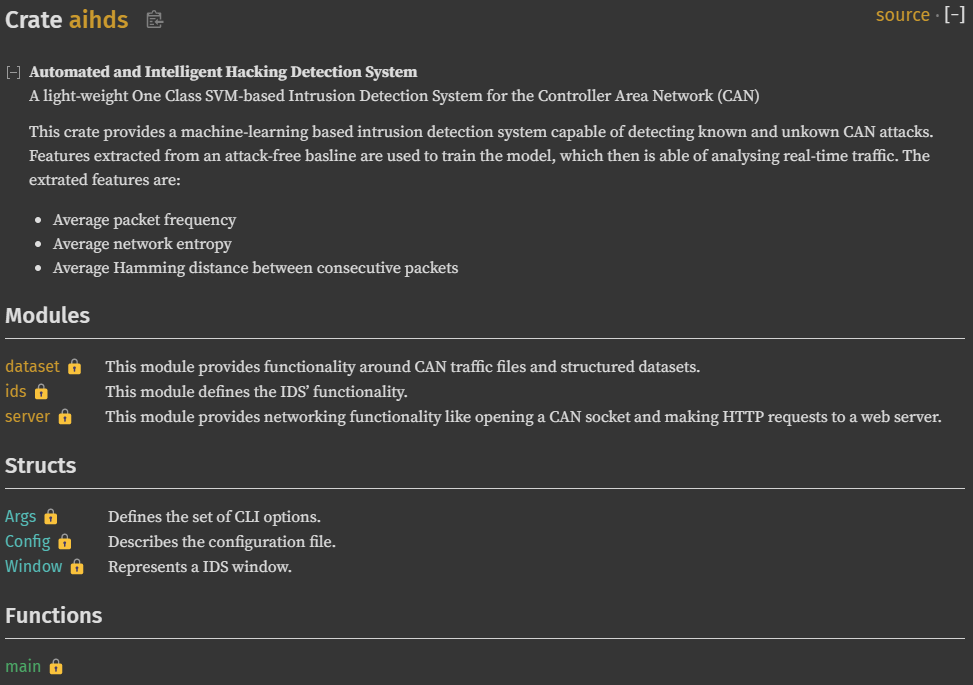
\includegraphics[width = \linewidth]{img/parts/docs/crate.png}
    \caption{Crate AIHDS}
    \label{fig:doc_crate}
\end{figure}

\begin{figure}
    \centering
    \begin{subfigure}[b]{\linewidth}
        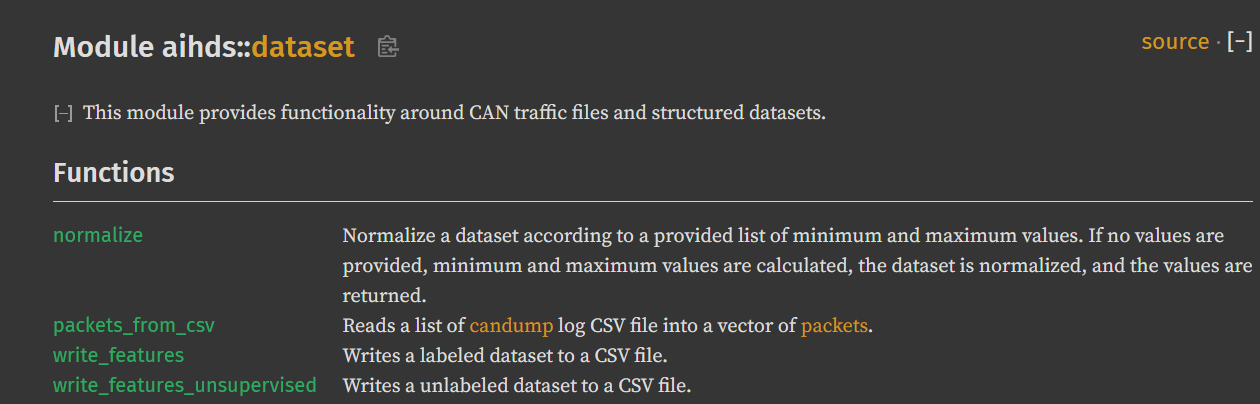
\includegraphics[width = \linewidth]{img/parts/docs/dataset/dataset.png}
        \caption{Module}
        \label{subfig:doc_dataset}
    \end{subfigure}
    \begin{subfigure}[b]{\linewidth}
        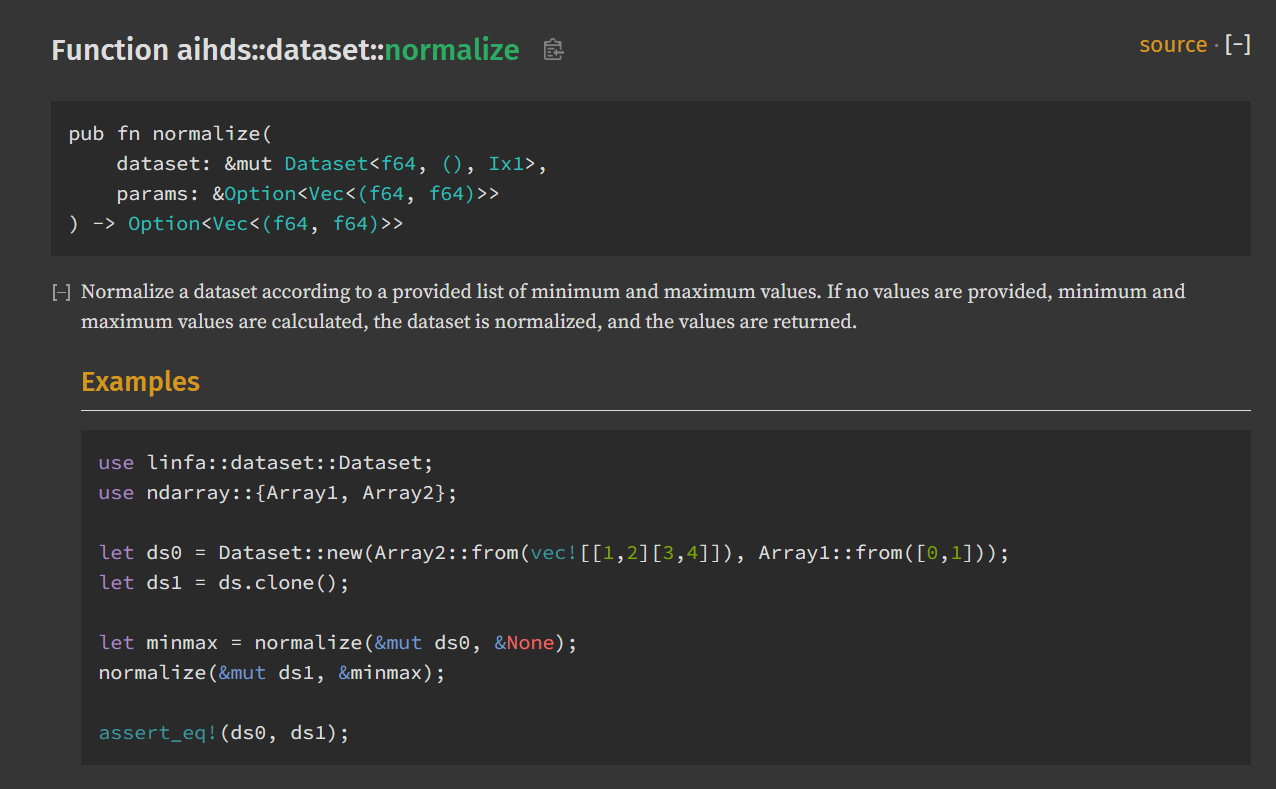
\includegraphics[width = \linewidth]{img/parts/docs/dataset/dataset_normalize.png}
        \caption{\emph{normalize} function}
        \label{subfig:doc_dataset_normalize}
    \end{subfigure}
    \begin{subfigure}[b]{\linewidth}
        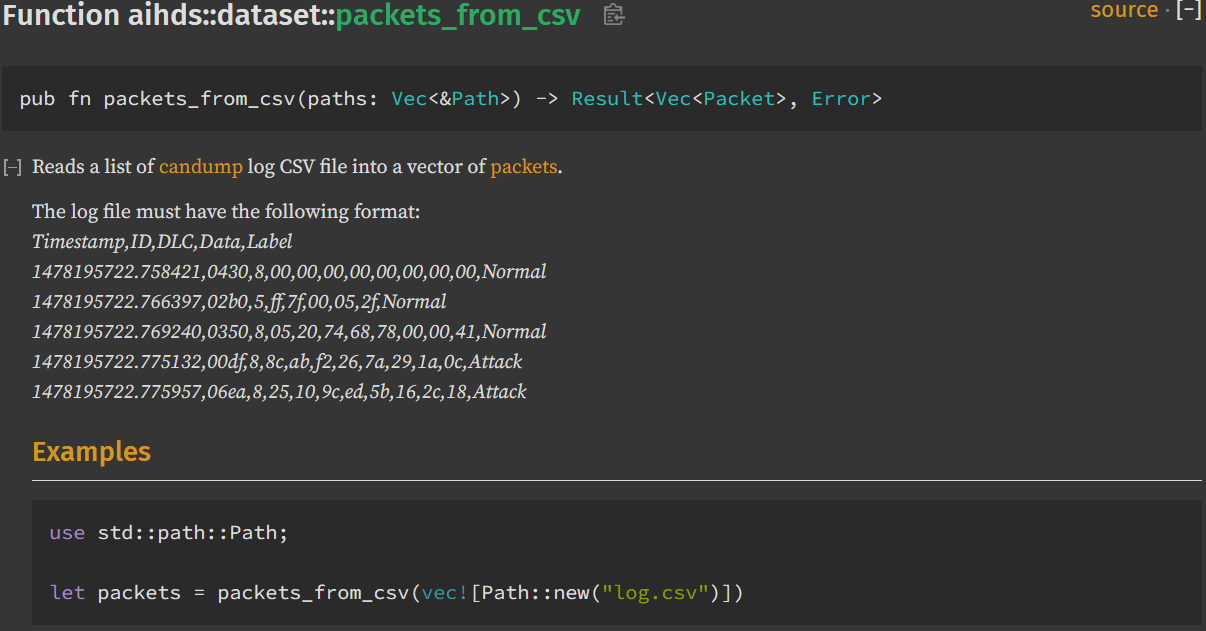
\includegraphics[width = \linewidth]{img/parts/docs/dataset/dataset_packetsfromcsv.png}
        \caption{\emph{packets\_from\_csv} function}
        \label{subfig:doc_dataset_packetsfromcsv}
    \end{subfigure}
    \caption{\emph{Dataset} module}
    \label{fig:doc_dataset}
\end{figure}
\begin{figure}
    \ContinuedFloat
    \begin{subfigure}[b]{\linewidth}
        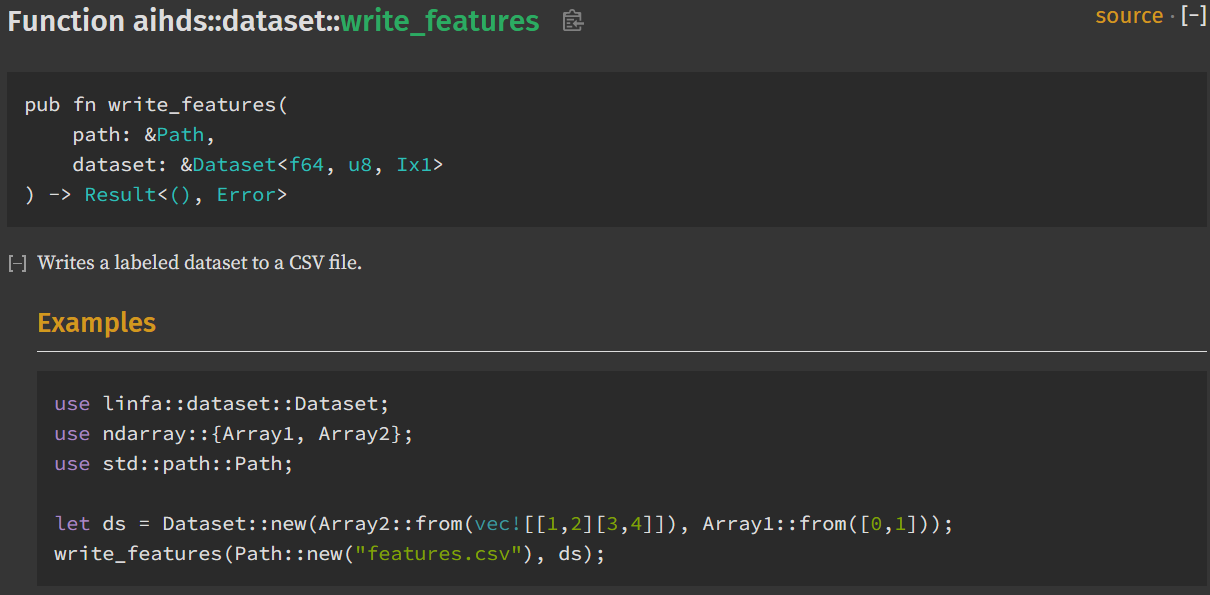
\includegraphics[width = \linewidth]{img/parts/docs/dataset/dataset_writefeatures.png}\
        \caption{\emph{write\_features} function}
        \label{subfig:doc_dataset_writefeatures}
    \end{subfigure}
    \begin{subfigure}[b]{\linewidth}
        \includegraphics[width = \linewidth]{img/parts/docs/dataset/dataset\_writefeaturesunsupervised.png}
        \caption{\emph{write\_features\_unsupervised} function}
        \label{subfig:doc_dataset_writefeaturesunsupervised}
    \end{subfigure}
    \caption{\emph{Dataset} module (cont.)}
    \label{fig:doc_dataset}
\end{figure}

\begin{figure}
    \centering
    \begin{subfigure}[b]{\linewidth}
        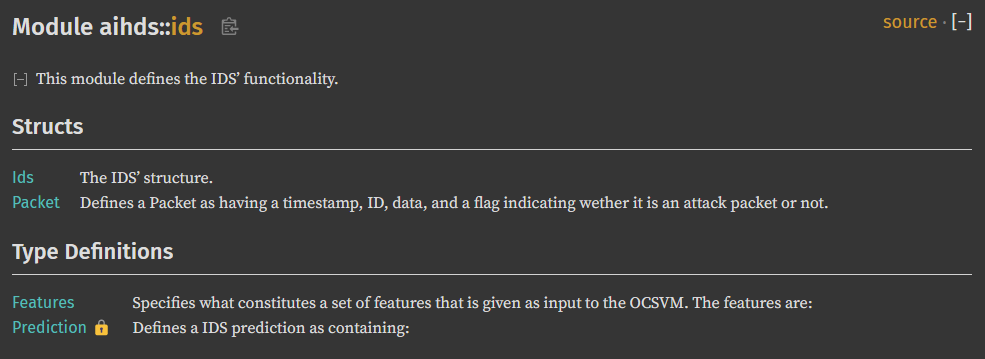
\includegraphics[width = \linewidth]{img/parts/docs/ids/ids.png}
        \caption{Module}
        \label{subfig:doc_ids}
    \end{subfigure}
    \begin{subfigure}[b]{\linewidth}
        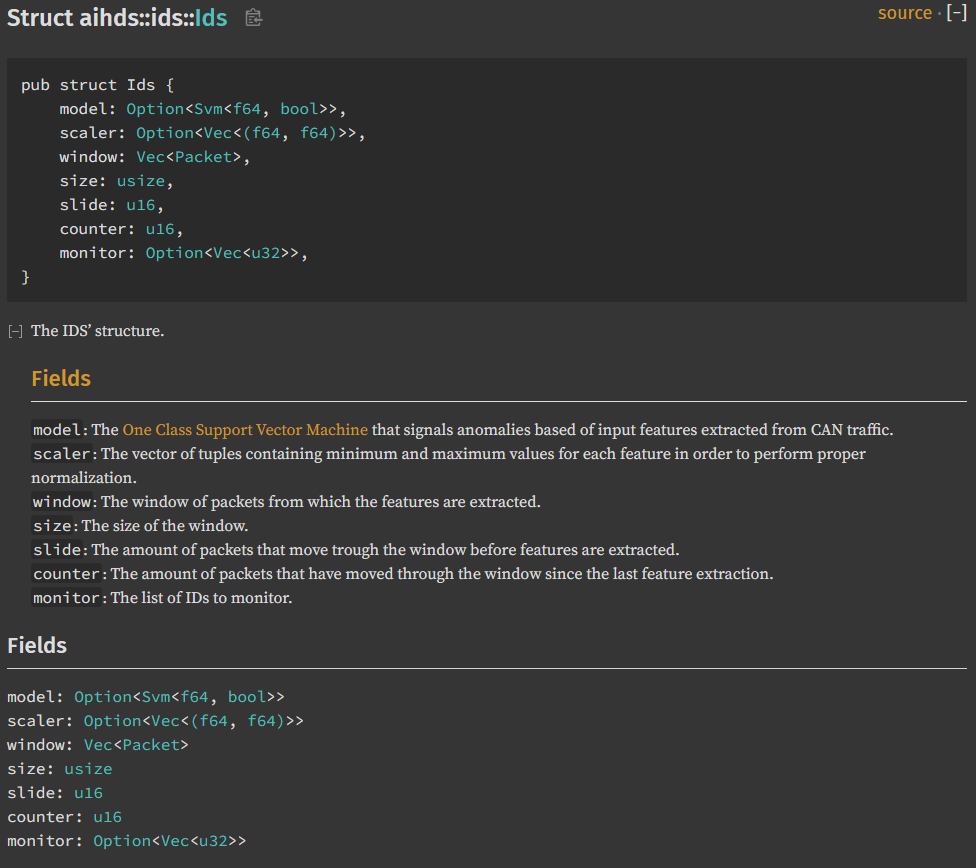
\includegraphics[width = \linewidth]{img/parts/docs/ids/ids_struct.png}
        \caption{Struct}
        \label{subfig:doc_ids_struct}
    \end{subfigure}
    \caption{\emph{IDS} module}
    \label{fig:doc_ids}
\end{figure}
\begin{figure}
    \ContinuedFloat
    \begin{subfigure}[b]{\linewidth}
        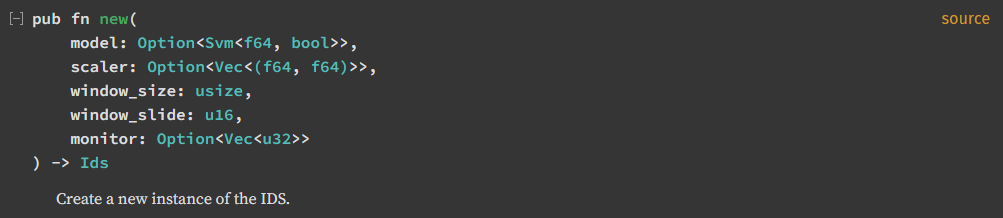
\includegraphics[width = \linewidth]{img/parts/docs/ids/ids_struct_new.png}
        \caption{IDS' \emph{new} function}
        \label{subfig:doc_ids_stuct_new}
    \end{subfigure}
    \begin{subfigure}[b]{\linewidth}
        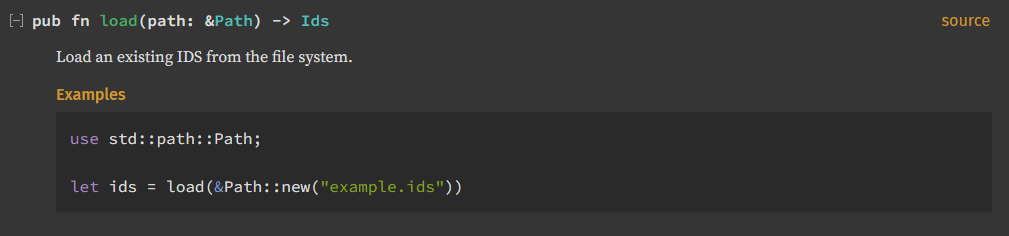
\includegraphics[width = \linewidth]{img/parts/docs/ids/ids_struct_load.png}
        \caption{\emph{load} function}
        \label{subfig:doc_ids_stuct_load}
    \end{subfigure}
    \begin{subfigure}[b]{\linewidth}
        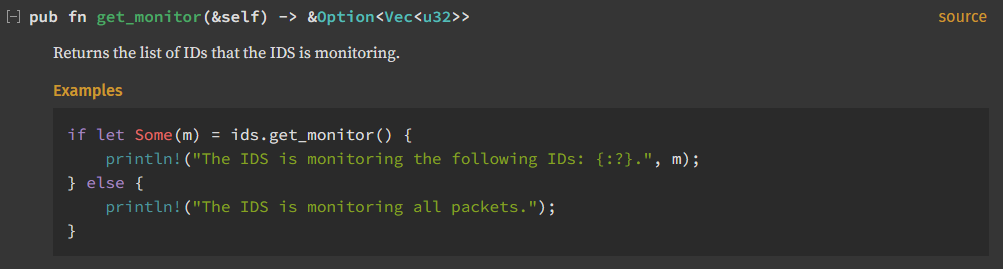
\includegraphics[width = \linewidth]{img/parts/docs/ids/ids_struct_getmonitor.png}
        \caption{\emph{get\_monitor} function}
        \label{subfig:doc_ids_stuct_getmonitor}
    \end{subfigure}
    \caption{\emph{IDS} module (cont.)}
    \label{fig:doc_ids}
\end{figure}
\begin{figure}
    \ContinuedFloat
    \begin{subfigure}[b]{\linewidth}
        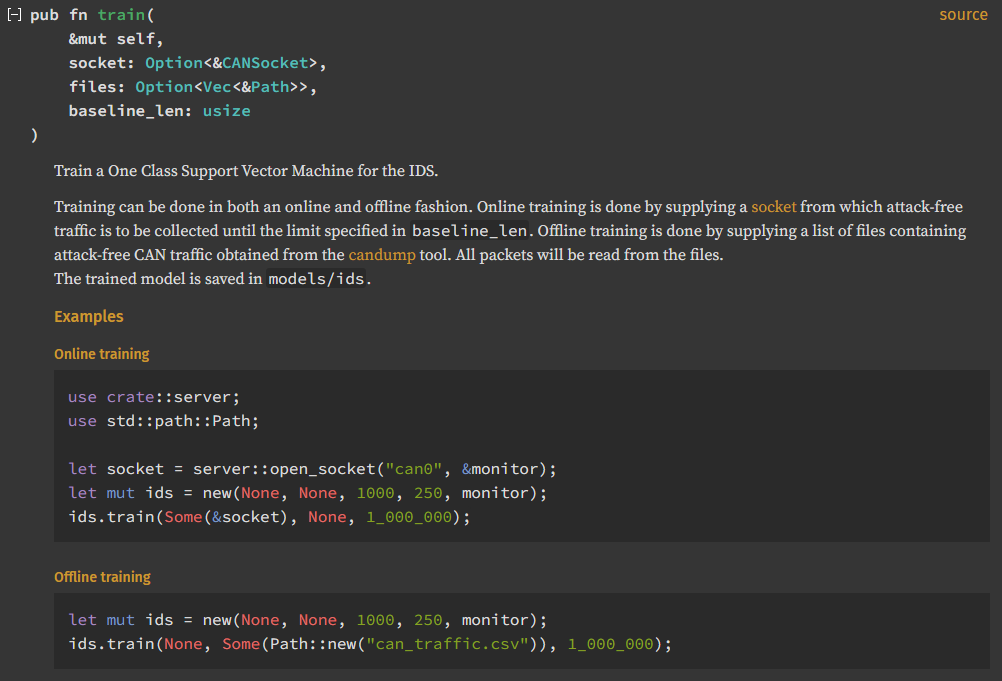
\includegraphics[width = \linewidth]{img/parts/docs/ids/ids_struct_train.png}
        \caption{\emph{train} function}
        \label{subfig:doc_ids_stuct_train}
    \end{subfigure}
    \begin{subfigure}[b]{\linewidth}
        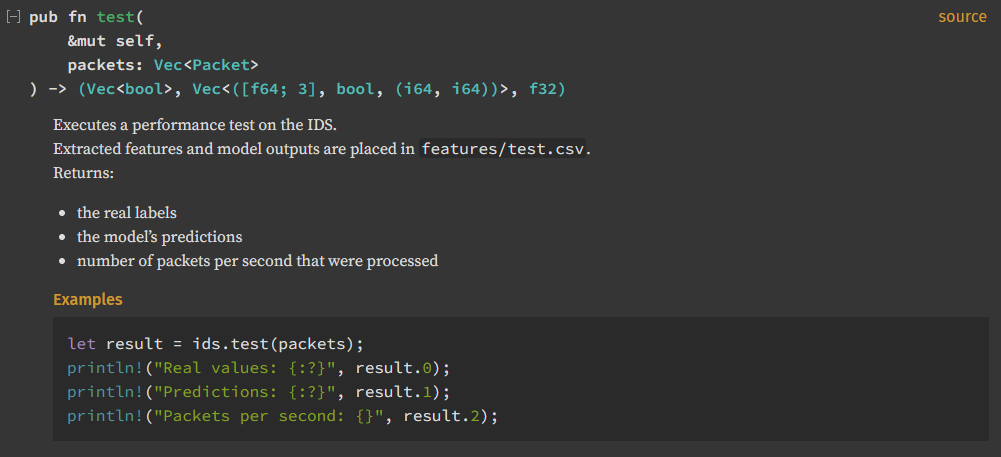
\includegraphics[width = \linewidth]{img/parts/docs/ids/ids_struct_test.png}
        \caption{\emph{test} function}
        \label{subfig:doc_ids_stuct_test}
    \end{subfigure}
    \caption{\emph{IDS} module (cont.)}
    \label{fig:doc_ids}
\end{figure}
\begin{figure}
    \ContinuedFloat
    \begin{subfigure}[b]{\linewidth}
        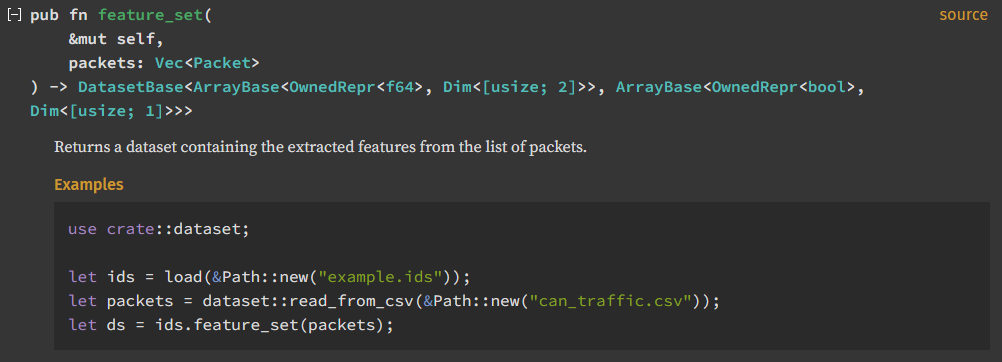
\includegraphics[width = \linewidth]{img/parts/docs/ids/ids_struct_featureset.png}
        \caption{\emph{feature\_set} function}
        \label{subfig:doc_ids_stuct_featureset}
    \end{subfigure}
    \begin{subfigure}[b]{\linewidth}
        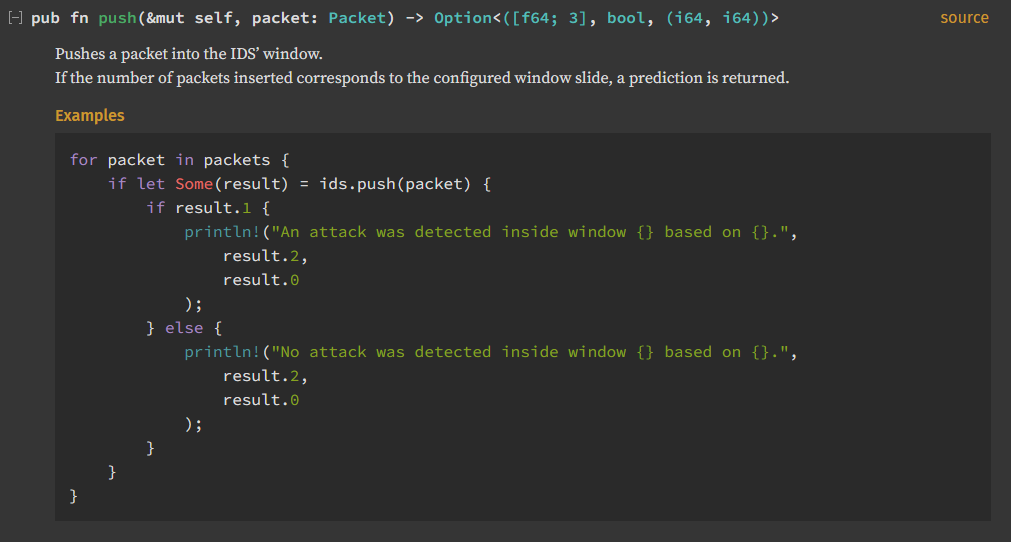
\includegraphics[width = \linewidth]{img/parts/docs/ids/ids_struct_push.png}
        \caption{\emph{push} function}
        \label{subfig:doc_ids_stuct_push}
    \end{subfigure}
    \begin{subfigure}[b]{\linewidth}
        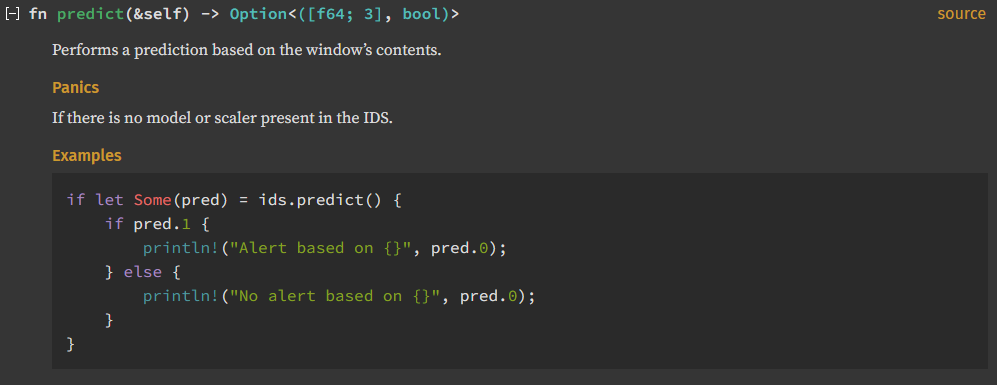
\includegraphics[width = \linewidth]{img/parts/docs/ids/ids_struct_predict.png}
        \caption{\emph{predict} function}
        \label{subfig:doc_ids_stuct_predict}
    \end{subfigure}
    \caption{\emph{IDS} module (cont.)}
    \label{fig:doc_ids}
\end{figure}
\begin{figure}
    \ContinuedFloat
    \begin{subfigure}[b]{\linewidth}
        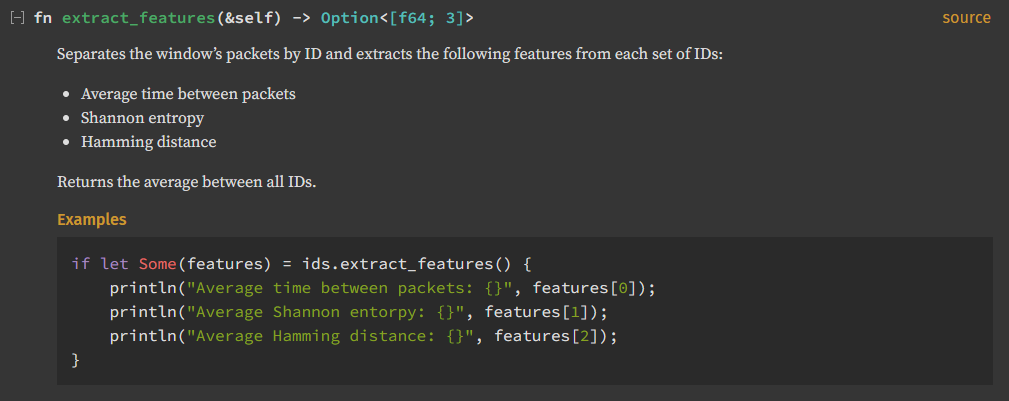
\includegraphics[width = \linewidth]{img/parts/docs/ids/ids_struct_extractfeatures.png}
        \caption{\emph{extract\_features} function}
        \label{subfig:doc_ids_stuct_extractfeatures}
    \end{subfigure}
    \begin{subfigure}[b]{\linewidth}
        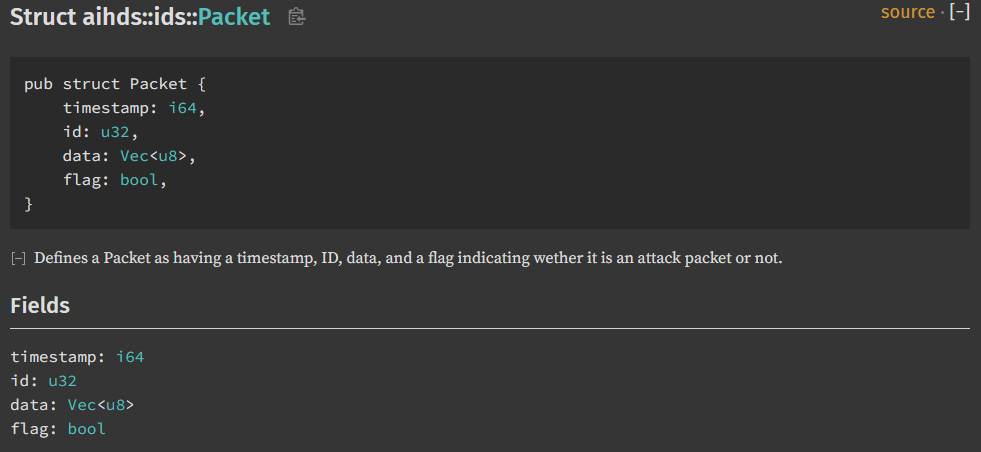
\includegraphics[width = \linewidth]{img/parts/docs/ids/packet_struct.png}
        \caption{\emph{Packet} struct}
        \label{subfig:doc_packet_struct}
    \end{subfigure}
    \begin{subfigure}[b]{\linewidth}
        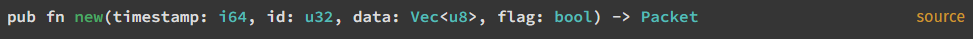
\includegraphics[width = \linewidth]{img/parts/docs/ids/packet_struct_new.png}
        \caption{Packet's \emph{new} function}
        \label{subfig:doc_packet_struct_new}
    \end{subfigure}
    \caption{\emph{IDS} module (cont.)}
    \label{fig:doc_ids}
\end{figure}
\begin{figure}
    \ContinuedFloat
    \begin{subfigure}[b]{\linewidth}
        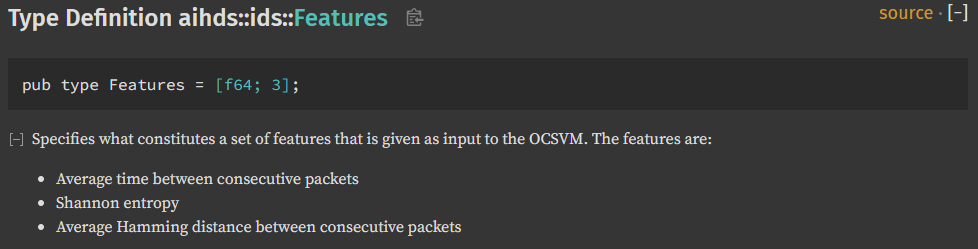
\includegraphics[width = \linewidth]{img/parts/docs/ids/ids_type_features.png}
        \caption{\emph{Features} type}
        \label{subfig:doc_ids_type_features}
    \end{subfigure}
    \begin{subfigure}[b]{\linewidth}
        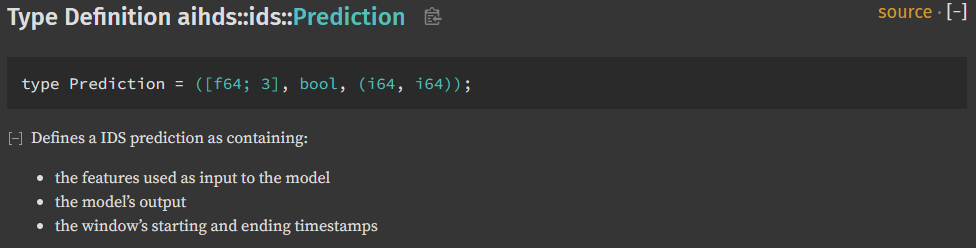
\includegraphics[width = \linewidth]{img/parts/docs/ids/ids_type_prediction.png}
        \caption{\emph{Prediction} type}
        \label{subfig:doc_ids_type_prediction}
    \end{subfigure}
    \caption{\emph{IDS} module (cont.)}
    \label{fig:doc_ids}
\end{figure}

\begin{figure}
    \centering
    \begin{subfigure}[b]{\linewidth}
        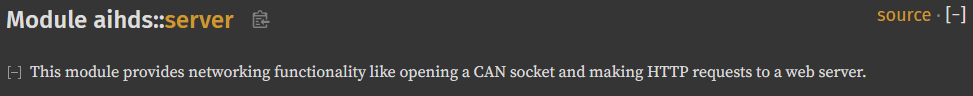
\includegraphics[width = \linewidth]{img/parts/docs/server/server.png}
        \caption{Module}
        \label{subfig:doc_server}
    \end{subfigure}
    \begin{subfigure}[b]{\linewidth}
        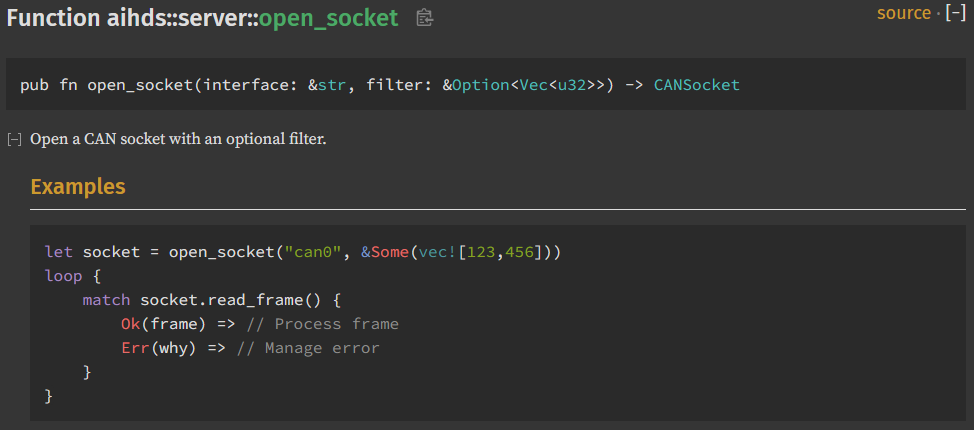
\includegraphics[width = \linewidth]{img/parts/docs/server/server_opensocket.png}
        \caption{\emph{open\_socket} function}
        \label{subfig:doc_server_opensocket}
    \end{subfigure}
    \begin{subfigure}[b]{\linewidth}
        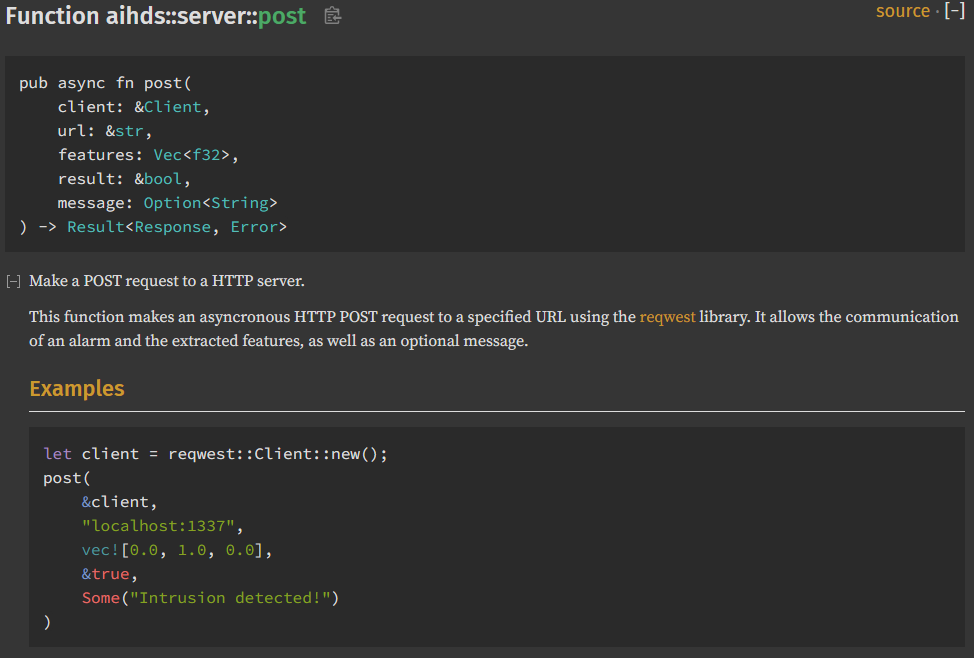
\includegraphics[width = \linewidth]{img/parts/docs/server/server_post.png}
        \caption{\emph{post} function}
        \label{subfig:doc_server_post}
    \end{subfigure}
    \caption{\emph{Server} module}
    \label{fig:doc_server}
\end{figure}